\documentclass[a4,12pt]{article}
\usepackage{fullpage}
\usepackage{graphicx}
\usepackage{url}
\usepackage{listings}

\newcounter{lst}[section]

\renewcommand{\thelst}{\arabic{section}.\arabic{lst}}

\lstnewenvironment{codelisting}[2]{
  \noindent        
  \label{code:#1}  
\lstset{language=#2,          
  basicstyle=\normalfont\scriptsize\sffamily,
  %breaklines=true,
%%%  basicstyle=\footnotesize,    
  xleftmargin=5pt,    
  mathescape=true,    
  frame=tb,    
  numbers=right,    
  numberstyle=\tiny,     
  stepnumber=1,     
  numbersep=-5pt}}{}

\lstnewenvironment{pythonlisting}{
  \noindent        
\lstset{language=python,          
  basicstyle=\normalfont\scriptsize\sffamily,
  %breaklines=true,
%%%  basicstyle=\footnotesize,    
  xleftmargin=5pt,    
  mathescape=true,    
  frame=tb,    
  numbers=right,    
  numberstyle=\tiny,     
  stepnumber=1,
  showstringspaces=false,
  numbersep=-5pt}}{}


 
\lstset{basicstyle=\sffamily}

\title{Artificial Intelligence Programming for Robots}

\begin{document}
\maketitle

This document forms a very basic tutorial for the BDIPython library.  Please note that this library is still very preliminary and under intermittent development.  There is no guarantee that this tutorial is up to date.

It is adapted from some Python programming exercises aimed at children in Year 9 in the UK so some of the instructions are quite basic - experienced Python programmers can probably skip some of the early sections on how to run IDLE and so on.  

We are going to explore programming robots using something called \emph{rational agent programming}.  In rational agent programming an \emph{agent} has \emph{beliefs} about the world and \emph{goals} it wants to achieve.  It uses \emph{rules} in order to decide what to do based on its beliefs and goals.

We will explore rational agent programming using a simulator of Pi2Go Robot.

\section{Setting up the Simulator}

Check clone \lstinline{pirover_simulator} from \url{https://github.com/legorovers/pirover_simulator}

In the \lstinline{pirover_simulator} folder you should find two files \lstinline{pysim.py} and \lstinline{pysimosx.py}.  The first is for use on Windows and Linux machines and the second for use on Macs.
You should run the simulator either from the command line or from a Python development environment such as IDLE.  

\begin{description}
\item[From the command line:]  Type \lstinline{python pysim.py} (\lstinline{pysimosx.py} on Macs) in the \lstinline{pirover_simulator} folder then press return.  

\item[From IDLE:] Start IDLE.  A window should open and you should see something like:
\end{description}

\begin{verbatim}
Python 3.7.2 (v3.7.2:9a3ffc0492, Dec 24 2018, 02:44:43) 
[Clang 6.0 (clang-600.0.57)] on darwin
Type "help", "copyright", "credits" or "license()" for more information.
>>>  
\end{verbatim}

Open \lstinline{pysim.py} (\lstinline{pysimosx.py} on Macs) from the File Menu.   A file will open in Idle (ignore this) and a new menu item {\bf Run} should appear.   From {\bf Run}  select {\bf Run Module}.

You should see:

\begin{center}
  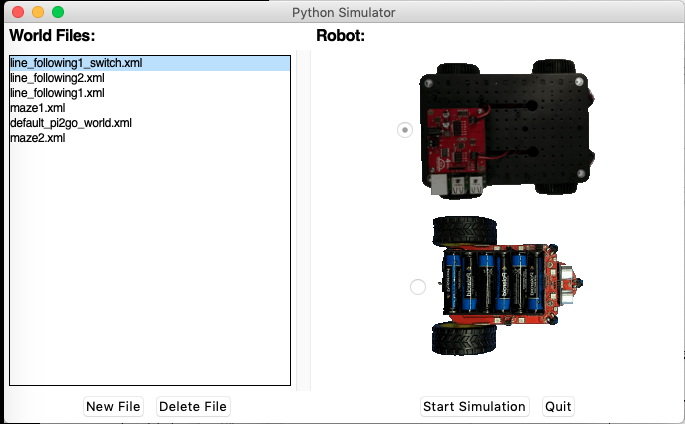
\includegraphics[width=14cm]{images/opening.png}
\end{center}

From here you can start a simulation for either the Initio robot (the top image) or the Pi2Go robot (the bottom image) in a number of settings (the “World Files” on the left).  

Select the Pi2Go robot and the \lstinline{default_pi2go_world.xml}
Then click on \emph{Start Simulation}

Once the simulation has started, you can stop it by pressing Q.

\subsection{Opening the Edit Window}

You can change the environment your virtual Pi2Go encounters by using objects from the Edit window.

Press E in the PiRover Simulator.  A second window, the Objects window, should open as shown in the screenshot below

\begin{center}
  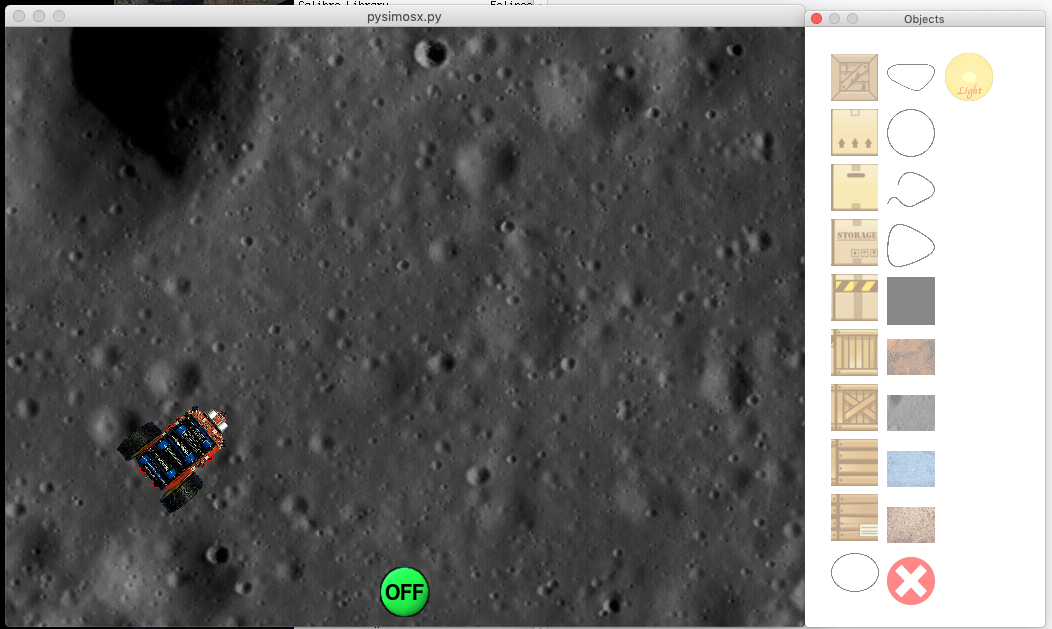
\includegraphics[width=14cm]{images/edit.png}
\end{center}

\subsection{Programming the Robot}

Open a new IDLE window or a new command line.  Try typing the following commands at the command line.

\begin{verbatim}
import simclient.simrobot as pi2go
pi2go.init()
pi2go.forward(10)
pi2go.stop()
\end{verbatim}


\section{BDIPython: Basics}
In rational agent programming an \emph{agent}, in this case your robot, acts according to various rules.  The agent continually checks which of its rules are applicable, picks one of them and then executes that rule.

\subsection{PYTHONPATH}

Make sure \lstinline{pirover_simulator} is on your PYTHONPATH.  In \lstinline{BDIPython} make sure \lstinline{BDIPython} itself is on your PYTHONPATH and \lstinline{BDIPython/tests}.

\subsection{Adding a Rule}
\label{sec:adding_a_rule}

\paragraph{Task} We will start programming with a very simple rule that is always applicable and which prints the input from a sensor to your screen.  We will start with the input from the small switch on the side of the real robot but displayed at the bottom of the simulator window.  This switch is shown in figure~\ref{fig:switch}.

\begin{figure}[htbp]
  \begin{center}
    
\includegraphics[width=3cm]{images/switch.png}
  \end{center}
  \caption{The Switch}
  \label{fig:switch}
\end{figure}

\begin{figure}[htbp]
\begin{pythonlisting}
import pi2goagent

agent = pi2goagent.Pi2GoAgent()

def print_switch_rule():
    switch_pressed = agent.sensor_value('switch_pressed')
    print("Switch Pressed: ", switch_pressed)
    return

agent.add_rule(print_switch_rule)
agent.run_agent()
\end{pythonlisting}
\caption{A First Agent Program}
\label{code:print_rule}
\end{figure}

\paragraph{Task} Copy program shown in figure~\ref{code:print_rule} into a file.   Save the file and run it.  

We will discuss each line of this program in turn.  Take some time to make sure you understand what it is doing.

\begin{description}
\item[Line 1]  First we import the Python code for the agent \lstinline{import pi2goagent}.
\item[Line 3] Then we create the \emph{agent} using \lstinline{agent = pi2goagent.Pi2GoAgent()}.  This creates the agent as a Python \emph{object}.  It isn't necessary for this tutorial to know much about Python objects.  They are much like other Python libraries and contain a number of functions which can be called using the \lstinline{agent.function()} syntax which you can see in lines 6, 10 and 11.  Unlike normal python libraries they can also contain data specific to the object, in this case a \emph{belief base} and a \emph{goal base} which we will discuss later.
\item[Line 5] Here we declare a Python \emph{function} called \lstinline{print_switch_rule}.  This represents our agent's rule.

  A Python function is defined with the keyword \lstinline{def} followed by the function name, brackets and then a colon.  On the line below and indented (like when using \lstinline{if}) are the Python commands to be executed by the function.  These are mostly just normal Python commands and should look familiar to you.

In this case the rule contains three lines of Python commands - on lines 6, 7 and 8 - which will be executed when the function is executed (in this case when the agent executes the rule).
\begin{sloppypar}
  \item[Line 6] Uses one of the agent's functions, \lstinline{agent.sensor_value(sensor_key)}.  This function returns the current value being sent by a particular sensor, in this case the switch.  This value is accessed using a string called the \emph{sensor key}.  This string is passed to the function as an \emph{argument}.  In the case of this program the sensor key is \lstinline{'switch_pressed'}.  So on this line we find the value of the the switch and store it in the Python variable \lstinline{switch_pressed}.
  \item[Line 7] prints out the value of the switch's sensor using Python's \lstinline{print command} and taking the value stored in \lstinline{switch_pressed}.
    \end{sloppypar}
\item [Line 8] The function ends by \emph{returning}.
\item[Line 10]  Here we add our rule to the agent.  \lstinline{agent.add_rule(rule_name)} is a function that takes the name of a rule as an argument.
\item[Line 11] Here we start the agent running.  \lstinline{agent.run_agent()} is a function that takes no arguments but starts the agent's \emph{reasoning cycle} which is discussed  next.
  \end{description}

\paragraph{Task}  Run your program using the \lstinline{python} command at the command line in your second tab.

\vspace{1cm}
\noindent What happens when the switch is pressed?
\medskip

\noindent You will need to use Ctrl-C to stop the program.

\newpage

\noindent All Pi2Go agent programs follow this basic format:
\begin{enumerate}
\item Create an agent object.
\item Define rules for the agent as python functions.
\item Add the rules to the agent.
\item Run the agent.
\end{enumerate}

When the agent runs it operates a \emph{reasoning cycle}.  The Pi2Go agent reasoning cycle is shown in figure~\ref{fig:reasoning_cycle}.
\begin{figure}[htbp]
  \begin{center}
    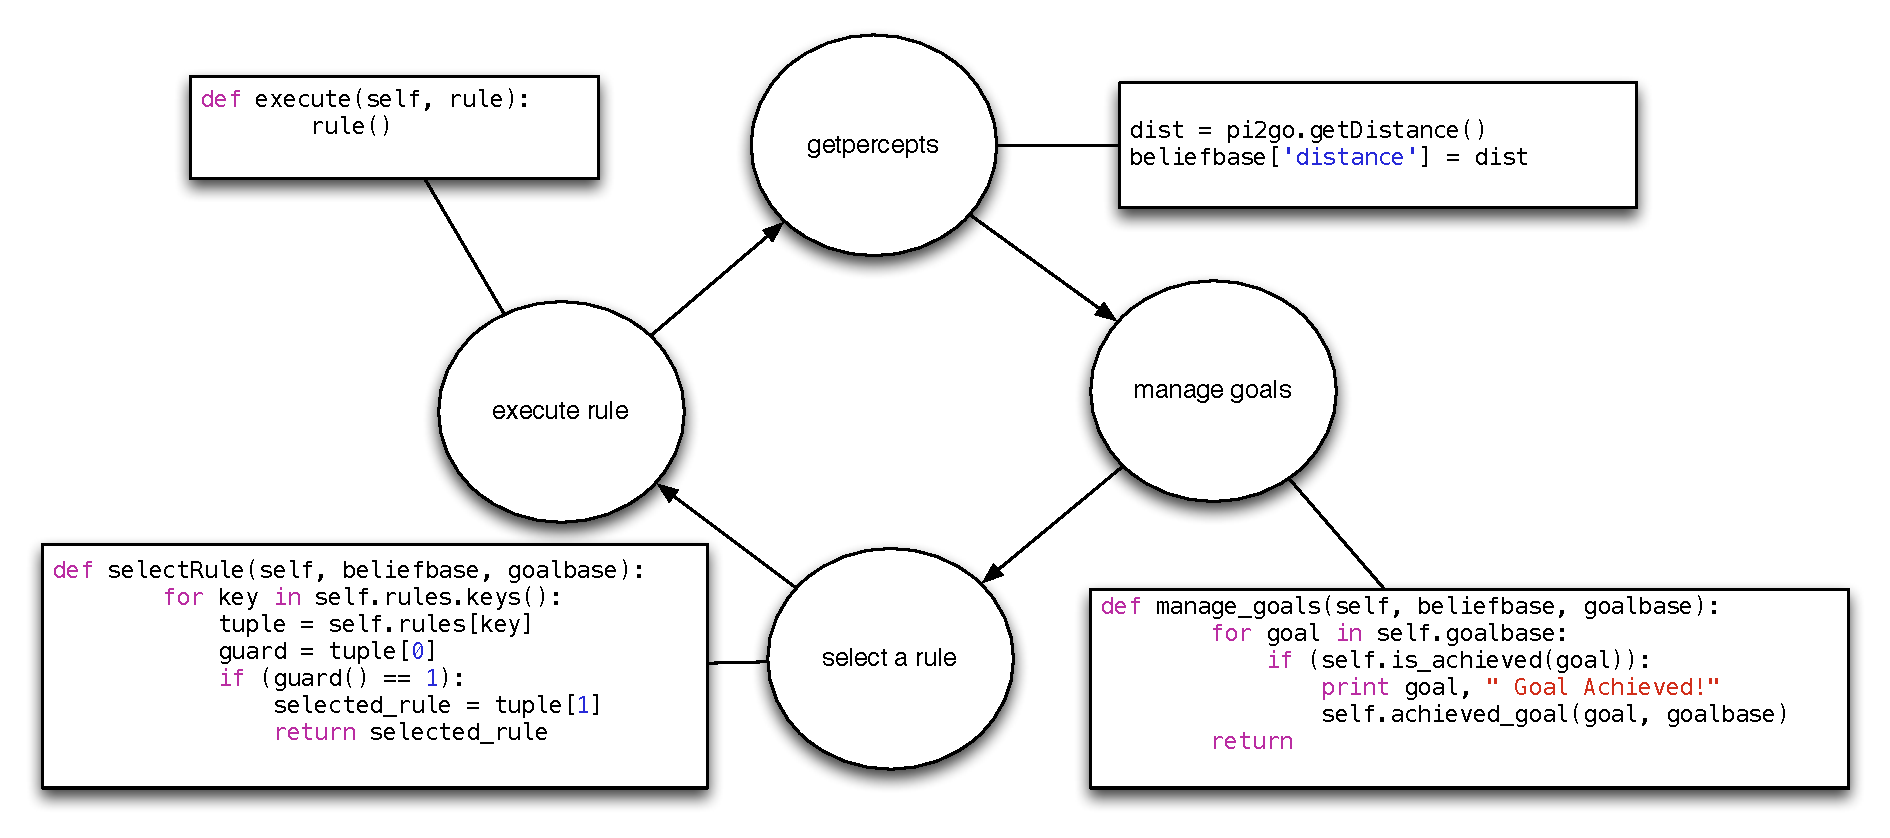
\includegraphics[width=14cm]{images/BDIPythonRC.pdf} 
  \end{center}
  \caption{The Pi2Go Agent Reasoning Cycle.  This starts by 1. checking all the sensors and updating the \emph{belief base} with values from the sensor.  2.  Checking all \emph{goals} and removing any that have been achieved (described in section~\ref{sec:goals}). 3. Checking all rules and picking the first that can be executed.  4.  Executes that rule or does nothing if no rules can be executed.}
  \label{fig:reasoning_cycle}
\end{figure}
The program in figure~\ref{code:print_rule} has only one rule.  So each time around the reasoning cycle that rule is executed and it prints out the current value of the switch sensor.

There are several other sensors.  Figure~\ref{fig:distance_sensors} shows the ones on the front of the robot.
\begin{figure}[htbp]
  \begin{center}
    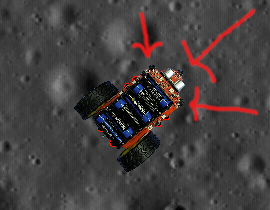
\includegraphics[width=7cm]{images/distance_sensors.png}
  \end{center}
  \caption{Sensors on the front of the robot.  There are three small \emph{infra red} sensors and a large \emph{ultrasonic} sensor at the front}
  \label{fig:distance_sensors}
\end{figure}
These sensors all operate in a similar way.  They emit something, either a pulse of infra red light (the three small sensors) or a pulse of ultrasonic noise (the large sensor), and then measure the value of the reflection or echo.

You can access the values returned by these sensors with the strings \lstinline{'obstacle_centre'}, \lstinline{'obstacle_left'}, \lstinline{'obstacle_right'} (the infra red sensors) and \lstinline{'distance'} (the distance sensor).

\paragraph{Task} Create a new python program by copying your first program to a new file and then modify this program so that the rule prints the value of a different sensor.  Check both \lstinline{'obstacle_centre'} and \lstinline{'distance'}.

\medskip

%% What is the sensor value when you place an object roughly 1cm, 3cm, 5cm and 10cm in front of the object with each of these sensors?
%% \begin{center}
%% \begin{tabular}{c|cccc}
%%  & 1cm & 3cm & 5cm & 10cm \\ \hline
%% \rule{0pt}{3ex} \lstinline{obstacle_centre}  & \underline{\hspace{3cm}} \quad & \underline{\hspace{3cm}} \quad & \underline{\hspace{3cm}} \quad & \underline{\hspace{3cm}} \quad\\
%% \lstinline{distance} & \underline{\hspace{3cm}} \quad & \underline{\hspace{3cm}} \quad & \underline{\hspace{3cm}} \quad & \underline{\hspace{3cm}} \quad
%% \end{tabular}
%% \end{center}


\subsection{Stopping the Program}

It is inelegant to use Ctrl-C to stop a program so instead we will use a sensor and a \emph{conditional rule}.

\paragraph{Task}  Create a Python function called \lstinline{stop_rule}, like \lstinline{print_switch_rule} in section~\ref{sec:adding_a_rule}.  Instead of calling \lstinline{agent.sensor_value(sensor_key)} this program should simply print the message \lstinline{"Stopping Agent"} and then (on the next line) call \lstinline{agent.done()} (this will stop the agent's reasoning cycle and so finish execution of your whole program).

You want this rule to be executed \emph{only if} the switch is pressed.  This means we need to add it as a \emph{conditional rule} to our agent.  The function \lstinline{agent.add_condition_rule(guard, rule_name)} adds a conditional rule to an agent.  This takes two arguments.  The first is a \emph{guard} which is a function that returns 1 (for true) and 0 (for false) when it is called.  The second argument is the name of a rule.

All the sensor values we looked at in section~\ref{sec:adding_a_rule} are stored in the agent's \emph{belief base}.  If the sensor returns either true or false (like \lstinline{'switch_pressed'} and \lstinline{'obstacle_centre'}) then they be accessed by calling the function \lstinline{agent.believe(sensor_key)} with the sensor's key string as an argument.  \lstinline{agent.believe(sensor_key)} returns the value 1 if the sensor is returning true and 0 if the sensor is returning false.

\begin{figure}[htbp]
  \begin{center}
    \fbox{\parbox{0.9\textwidth}{\vspace{-0.3cm}\paragraph{Side Note for the Curious}  We can't use \lstinline{agent.sensor_value(sensor_key)} as a guard because it will store the value of the function \emph{at the time the rule is added to the robot} while \lstinline{agent.believe(sensor_key)} waits until the rule is executed before checking the value.  Delaying the execution of a python function is quite advanced programming and you do not need to understand how this works here.  Normally it can be achieved just by passing the name of one function as an argument to another (this is why we use rule names as arguments in \lstinline{agent.add_rule(rule_name)} and \lstinline{agent.add_condition_rule(guard, rule_name)}) but it is complicated in \lstinline{agent.believe(sensor_key)} by the fact the function takes the sensor key as an argument.}}
    \end{center}
\end{figure}


So, assuming your stop rule is called \lstinline{stop_rule}, you add a conditional rule that the agent should stop if the switch is pressed by writing:

\medskip
\lstinline{agent.add_condition_rule(agent.believe('switch_pressed'), stop_rule)}
\medskip

{\bf Important:}  The conditional rule needs to be added \emph{before} the print sensor value rule.  This is because the agent always executes picks the first rule that applies in the order that they were added.

%% \medskip

%% What do you think would happen if the conditional rule were added second?
%% \nopagebreak
%% \vspace{1cm}
%% \hrule
%% \vspace{1cm}
%% \hrule
%% \medskip

\paragraph{Task} Create a program which prints out the readings from one sensor until the switch is pressed.

\subsection{Moving the Robot}
\label{sec:moving}

We will now get the robot to drive forwards until the switch is pressed.  For this you will need to replace your print sensor rule with a go forward rule.

To make the robot go forwards you want to use a function contained in the robot's library rather than in the agent object.  In order to to this you need to import \lstinline{simclient.simrobot as pi2go} as well as \lstinline{pi2goagent} at the start of your program.   This is a normal library so you do not need to create any objects.  

\paragraph{Task} Use \lstinline{pi2go.forward(20)} to create a program where the robot moves forwards at speed 20 until the switch is pressed.  Use a rule that first prints the message \lstinline{Going Forward} and then moves the robot.  You may want to include the command \lstinline{pi2go.stop()} in your stop rule.  This stops the Pi2Go's motors.

\subsection{Using Internal Beliefs to Control Rules}

You will have noticed in section~\ref{sec:moving} that the robot keeps printing \lstinline{Going Forward}.  This is because the rule is selected and executed on each turn of the reasoning cycle.  It would be better if the rule is executed just once, to start the robot moving and isn't executed again.  Ideally we would like to use a conditional rule with the guard that the robot believes it isn't moving.

To do this we will need to add an \emph{internal belief} to the belief base.  The agent function for adding internal beliefs is shown in line 2 of figure~\ref{code:forward_rule}.
\begin{figure}[htbp]
\begin{pythonlisting}
def forward_rule():
       agent.add_belief('moving')
       pi2go.forward(20)
       return
\end{pythonlisting}
\caption{A Rule that adds an Internal Belief}
\label{code:forward_rule}
\end{figure}

We only want the agent to move if we \emph{don't believe} we are moving.  We can create our guard using the function \lstinline{agent.NOT(belief)} -- i.e.,
\begin{itemize}
\item \lstinline{agent.NOT(agent.believe('moving'))} or
\item \lstinline{agent.NOT(agent.B('moving'))}
\end{itemize}

{\bf NB:}  \lstinline{agent.B} is a shortened form of \lstinline{agent.believe}.

\paragraph{Task}  Write a program to make your start moving forward until the switch is pressed.  This program should only start the robot moving once.

%% \vspace{1cm}
%% \noindent What do you think could improve this program?: \underline{\hspace{7.5cm}}
%% \vspace{1cm}
%% \hrule
%% \medskip

\subsection{Using the Switch to Start and Stop Operation}

You are probably becoming frustrated by the way the keyboard and monitor make it difficult to move the robot properly.  

Instead of just using the switch to stop the robot program we could also use it to start the program by getting it to add an internal belief \lstinline{started} and a rule for starting.  This will let you delay the start of robot motion in order to give you time to unplug the keyboard, mouse and monitor and let the robot move about.

However, if you have unplugged the monitor you will no longer be able to use a print statement to tell if the agent has noticed your switch press (sometimes if you press and release too quickly it can miss the switch press).  Fortunately the Pi2Go has a set of LEDs around it which can light up in various different colours.

\begin{figure}[htbp]
\begin{pythonlisting}
def start_rule():
	print "Starting Agent"
	agent.add_belief('started')
	pi2go.setAllLEDs(4095, 4095, 4095)
	time.sleep(1)
	pi2go.setAllLEDs(0, 0, 0)
	return
\end{pythonlisting}
\caption{A Start Rule that flashes the LEDs white when a switch press is detected.}
\label{code:start_rule}
\end{figure}

Figure~\ref{code:start_rule} shows a start rule that adds the belief \lstinline{'started'} in line 3.  In line 4 the rule calls the function \lstinline{setAllLEDs}.  This takes three arguments for the value of the red, green and blue light to be displayed.  We are passing in the maximum for all three values which gives us a bright white light, but many other colours can be displayed by changing the numbers.  We then get the rule to sleep for a millisecond using \lstinline{time.sleep(1)}. {\bf Important:} for this you will need to import the \lstinline{time} library.  Then it sets the value of all LEDs to 0 (i.e., switches all the lights off).  Figure~\ref{fig:leds} lists the functions for controlling the Pi2Go LEDs and these are also listed at the end of this booklet.

\begin{figure}[htbp]
\hrule
\begin{description}
\item[setLED(LED, Red, Green, Blue)] Sets the LED specified to required RGB value.  $1 \leq LED \leq 4$, $0 \leq Red, Green, Blue \leq 4095$
\item[setAllLEDs(Red, Green, Blue)] Sets all LEDs to required RGB.   $0 \leq Red, Green, Blue \leq 4095$
\end{description}
\hrule
\caption{Pi2Go LED Functions}
\label{fig:leds}
\end{figure}

The sleep function isn't included just to allow the flash of light to be seen.  You also want time to release the switch before the agent checks again otherwise it will instantly execute the stop rule.

We want
\begin{itemize}
\item The agent to start if it \underline{believes} the switch is pressed and \underline{doesn't believe} it has started.
\item We want the agent to move it if \underline{believes} it has started and \underline{doesn't believe} it is already moving.
  \item We want the agent to stop if it \underline{believes} it has started and \underline{believes} the switch is pressed.
\end{itemize}

We can use \lstinline{agent.AND(belief1, belief2)} along with \lstinline{agent.NOT(belief)} in order to create the guards we need.

If you feel your calls to \lstinline{agent.add_condition_rule(guard, rule_name)} are getting very long (this is particularly irritating with a small monitor) then you can use python variables just as in a normal python program.  You can see an example of this in figure~\ref{code:variables}

\begin{figure}[htbp]
  \begin{pythonlisting}
b_switch = agent.B('switch_pressed')
b_started = agent.B('started')
b_moving = agent.B('moving')

b_ready_to_start = agent.AND(b_switch, agent.NOT(b_started))
b_ready_to_move = agent.AND(b_started, agent.NOT(b_moving))
b_ready_to_stop = agent.AND(b_switch, b_started)

agent.add_condition_rule(b_ready_to_start, start_rule)
agent.add_condition_rule(b_ready_to_move, forward_rule)
agent.add_condition_rule(b_ready_to_stop, stop_rule)
agent.run_agent()
  \end{pythonlisting}
  \caption{Using Python variables for complex conditions}
  \label{code:variables}
\end{figure}

\paragraph{Task} Write a program for your Pi2Go so that when the switch is pressed it starts moving forwards and when the switch is pressed again it stops executing.

\subsection{Summary}
This section has used several very simple programs to illustrate the basics of rational agent programming using the Pi2Go.  It has introduced the \lstinline{agent} object and illustrated several useful functions.  There are two further functions that you will need in the next sections.

\begin{description}
\item[agent.drop\_belief(belief)] This function allows you to drop an internal belief.  This can be important if you have, for instance, several different types of moving behaviour you want to switch between and the agent needs to know which one it is using at the moment.
  \item[agent.OR(belief1, belief2)] is used in guards.  This returns true if the agent believes \emph{either} \lstinline{belief1} or \lstinline{belief2}.
\end{description}

Figure~\ref{fig:agent_functions} summarises all the agent functions.  Figure~\ref{fig:sensor_keys} summarises the sensor keys.  Note that some of these functions and sensor keys have not been introduced yet.  They will be described when you need them.

\begin{figure}[htbp]
  \hrule
  \begin{description}
\item[agent.sensor\_value(sensor\_key)] Returns the value of the sensor associated with \lstinline{sensor_key}.
\item[agent.add\_belief(belief)] Adds an internal belief.
\item[agent.drop\_belief(belief)] Removes an internal belief.
  \item[agent.believe(belief\_key)] Returns true if the agent believes \lstinline{belief}.
  \item[agent.B(belief\_key)] Returns true if the agent believes \lstinline{belief}.
  \item[agent.AND(belief1, belief2)] This returns true if the agent believes \emph{both} \lstinline{belief1} and \lstinline{belief2}.
  \item[agent.OR(belief1, belief2)] This returns true if the agent believes \emph{either} \lstinline{belief1} or \lstinline{belief2}.
  \item[agent.NOT(belief)] This returns true if the agent doesn't belief \lstinline{belief}
 \item[agent.add\_goal(goal)] Adds a goal to the agent's goal base.
 \item[agent.drop\_goal(goal)] Removes a goal from the agent's goal base.
 \item[agent.has\_goal(goal)] Returns true if the agent has goal \lstinline{goal}.
 \item[agent.G(goal)] Returns true if the agent has goal \lstinline{goal}.
 \item[agent.goal\_is\_achieved\_when(goal, belief)] Tells the agent what must be believed for \lstinline{goal} to be achieved.
 \item[agent.add\_rule(rule\_name)] Adds an unconditional rule to the agent.
 \item[agent.add\_condition\_rule(guard, rule\_name)] Adds a conditional rule to the agent with guard, \lstinline{guard}.
 \item[agent.run\_agent()] Starts the agent's reasoning cycle.
 \item[agent.done()] Stops the agent's reasoning cycle.
  \end{description}
  \hrule
  \caption{Summary of all the functions of the agent object}
  \label{fig:agent_functions}
\end{figure}


\begin{figure}[htbp]
  \hrule
  \begin{description}
  \item[switch\_pressed] True if the switch is pressed, false otherwise.
  \item[obstacle\_centre] True if something is close to the front infra red sensor.
  \item[obstacle\_right] True if something is close to the front right infra red sensor.
  \item[obstacle\_left] True if something is close to the front left infra red sensor.
  \item[distance] Returns the distance something is in front of the ultrasonic sensor.
    \item[no\_line\_left] True if there is a bright colour beneath the left downward pointing infra red sensor.
    \item[no\_line\_right] True if there is a bright colour beneath the right downward pointing infra red sensor.
      \item[lightFL] Returns the light intensity recorded by the front left light sensor.
      \item[lightFR] Returns the light intensity recorded by the front right light sensor.
      \item[lightBL] Returns the light intensity recorded by the back left light sensor.
      \item[lightBR] Returns the light intensity recorded by the back right light sensor.
  \end{description}
  \hrule
  \caption{Summary of all the Sensor Keys}
  \label{fig:sensor_keys}
\end{figure}


\section{Obstacle Avoidance Behaviour}

You are now ready to start programming some more complex behaviours for the robot.

As well as \lstinline{forward} the \lstinline{pi2go} library has a number of other functions for moving the robot.  These are summarised in figure~\ref{fig:move_functions}.

\begin{figure}[htbp]
  \hrule
\begin{sloppypar}
\begin{description}
\item[stop()] Stops both motors
\item[forward(speed)] Sets both motors to move forward at speed. $0 \leq speed \leq 100$
\item[reverse(speed)] Sets both motors to reverse at speed. $0 \leq speed \leq 100$
\item[spinLeft(speed)] Sets motors to turn opposite directions at speed. $0 \leq speed \leq 100$
\item[spinRight(speed)] Sets motors to turn opposite directions at speed. $0 \leq speed \leq 100$
\item[turnForward(leftSpeed, rightSpeed)] Moves forwards in an arc by setting different speeds. $0 \leq leftSpeed, rightSpeed \leq 100$
\item[turnreverse(leftSpeed, rightSpeed)] Moves backwards in an arc by setting different speeds. $0 \leq leftSpeed, rightSpeed \leq 100$
\item[go(leftSpeed, rightSpeed)] controls motors in both directions independently using different positive/negative speeds. $-100\leq leftSpeed, rightSpeed \leq 100$
\item[go(speed)] controls motors in both directions together with positive/negative speed parameter. $-100\leq speed \leq 100$
\end{description}
\end{sloppypar}
\hrule
\caption{Summary of the Pi2Go Movement Functions}
\label{fig:move_functions}
\end{figure}

\paragraph{Task} Program the robot so that if it believes there is an obstacle in front of any of its infra-red sensors it turns until there is no longer an obstacle, at which point it carries on moving forwards.  You may want to use \lstinline{agent.OR(belief1, belief2)} to construct the guard for your rules and \lstinline{agent.drop_belief(belief)} to help the robot know whether it is moving forwards or turning.

\paragraph{Option} Customise this program so that the direction in which the robot turns depends upon which sensors are detecting the obstacle so that it turns in the most sensible direction to clear the obstacle depending upon whether it is on the right or on the left.

\section{Abstractions:  Light Following Behaviour}

So far we have been able to directly use the beliefs that come in from sensors, but now we are going to look at the light sensors which do not return \lstinline{True} or \lstinline{False} but a number between 0 and 1023 depending upon how strong a light they are detecting.

The light sensors are contained in the two LEDs at the front and at the back of the robot.  They can be accessed with the sensor keys \lstinline{'lightFL'} (front left), \lstinline{'lightFR'} (front right), \lstinline{'lightBL'} (back left), \lstinline{'lightBR'} (back right).

To use these as beliefs we are going to have to define \emph{abstractions} from these values to the ``true'' and ``false'' used by beliefs.  To do this we will define them as Python functions which return either 1 (for true) or 0 (for false).

Figure~\ref{code:light} defines a function \lstinline{b_light_on_front_right} which represents that the belief that there is a brighter light on the right at the front of the robot than on the left.  It does this getting the sensor values from the front two light sensors and comparing them.  If \lstinline{lightFR} is greater than \lstinline{lightFL} by 10 then it believes the light is brighter on the right.

\begin{figure}[htbp]
\begin{pythonlisting}
def b_light_on_front_right():
	lightFL = agent.sensor_value('lightFL')
	lightFR = agent.sensor_value('lightFR')
	print "Left Light: ", lightFL, "Right Light: ", lightFR
	if (lightFL < lightFR and lightFR - lightFL > 10):
		return 1
\end{pythonlisting}
\caption{A Python Function that abstracts values from the Light Sensors}
\label{code:light}
\end{figure}

To add a conditional rule to a program that will make the robot turn towards the right if the light is brighter on that side then you add the \emph{name of} the function as the guard.  For instance:

\medskip

\lstinline{agent.add_condition_rule(b_light_on_front_right, turn_right_rule)}

\medskip

\begin{sloppypar}
\noindent The name of the function can also be used with the functions \lstinline{agent.AND(belief1, belief2)}, \lstinline{agent.OR(belief1, belief2)} and \lstinline{agent.NOT(belief)}.  For instance:
\end{sloppypar}


\medskip

\lstinline{agent.AND(b_light_on_front_right, agent.B('started'))}

\medskip

\noindent represents the condition that the light is brighter at the front \emph{and} the robot has started.

\paragraph{Task} Program the robot to turn on the spot so that it faces the brightest light in the room.  Create abstractions using all four light sensors to achieve this.

\paragraph{Option} Modify your program so that the robot drives towards the brightest light in the room.  If the light is moving it should follow the light.  You may want to use \lstinline{turnForward} instead of \lstinline{spinLeft} and \lstinline{spinRight}.

\paragraph{Option} Go back to your obstacle avoidance program and adapt it to use the ultrasonic distance sensor, so that it detects obstacles sooner.

\section{Line Following Behaviour}

The Pi2Go has two additional infrared sensors underneath the robot.  Since they are pointing downwards they measure how much light is reflected from the floor and this depends upon what colour the floor is.  The sensors return \lstinline{True} if the floor is a light colour (such as white) and \lstinline{False} if it is a dark colour (such as black).  These sensor values are returned with the keys \lstinline{'no_line_left'} (to indicate a light colour on the left) and \lstinline{'no_line_right'} (to indicate a light colour on the right).

This means if you place the robot so the two sensors are either side of a thick black line it should be able to travel along the line by moving forwards (when neither sensor detects the line) and turning left or right (as appropriate) when one of the sensors detects the line.

\paragraph{Task} Program your robot to follow a line.

\section{Goal Directed Behaviour}
\label{sec:goals}

So far the agents have been working only with beliefs.  To get more complex behaviour it is necessary to consider what the robot is trying to do.  Rational agent programming uses the idea of a \emph{goal} that the agent is trying to achieve to represent this.

The Pi2Go Agent has several functions that support programming with goals:

\begin{description}
\item[agent.add\_goal(goal\_key)] This adds a goal to the agent's \emph{goal base}
\item[agent.has\_goal(goal\_key)] Is used in rule guards to detect whether the agent has a goal.
\item[agent.G(goal\_key)] is identical to \lstinline{agent.has_goal(goal_key)}
\end{description}

A goal remains in the agent's goal base until it is believed to be true.  So, in a simple case, if our goal key is the same as one of the sensor keys the then agent will continue to have that goal until that sensor returns \lstinline{True}.

\paragraph{Task}  Write a program which adds the goal \lstinline{'obstacle_centre'} during the start rule (this is the \emph{initial goal}).  The program should have a rule that makes the robot drive forwards if it has started and has the goal \lstinline{'obstacle_centre'}.

\subsection{Complex Goals}

The function \lstinline{agent.goal_is_achieved_when(goal_key, belief)} can link a goal key with a complex belief allowing you to create more complex goals.

Consider the python code

\noindent \begin{pythonlisting}
b_obstacle = agent.OR(b_obstacle_centre, agent.OR(b_obstacle_left, b_obstacle_right))

agent.goal_is_achieved_when('obstacle', b_obstacle)
\end{pythonlisting}

\vspace{1cm}
\noindent What do you think this code does? \underline{\hspace{10cm}}
\vspace{1cm}
\hrule
\medskip

\paragraph{Task}  Adapt your previous program to use \lstinline{'obstacle'} as the goal rather than \lstinline{'obstacle_centre'}.

\subsection{Abstract Goals}

\lstinline{agent.goal_is_achieved_when(goal_key, belief)} can also be used to define abstract goals using functions.   Consider

\noindent \begin{pythonlisting}
def b_in_the_light():
	lightFL = agent.sensor_value('lightFL')
	lightFR = agent.sensor_value('lightFR')
	if (lightFL > 250 and lightFR > 250):
		return 1
	return 0

agent.goal_is_achieved_when('in_the_light', b_in_the_light)
\end{pythonlisting}

\vspace{1cm}
\noindent What do you think this code does? \underline{\hspace{10cm}}
\vspace{1cm}
\hrule
\medskip

\paragraph{Task} Write a program to make a robot drive to a very bright part of the room and then stop.

\subsection{Subgoals}

A robot can have multiple goals at once.  This allows you to use some goals as \emph{subgoals}.  For instance a robot with a goal to find an obstacle might need to find a line first and then follow that line to the obstacle.  So the first thing it does, if it has a goal to find an obstacle is set up a subgoal to fine a line (e.g., by driving forwards).  Once that subgoal is achieved then it can start line following behaviour to find the obstacle.

\paragraph{Task} Write a program to find a line and then follow it until it meets an obstacle.

\section{More Complex Programs for you to try}

\paragraph{Task}  Write a program to drive to a very bright part of the room, then follow a line until it meets an obstacle.

\paragraph{Task} Write a program where an agent in a very bright part of the room gets a goal to find an obstacle, and an agent that has found an obstacle gets a goal to move to a very bright part of the room.

\section{Command Summaries}

\subsection{LED Functions}

\begin{description}
\item[setLED(LED, Red, Green, Blue)] Sets the LED specified to required RGB value.  $1 \leq LED \leq 4$, $0 \leq Red, Green, Blue \leq 4095$
\item[setAllLEDs(Red, Green, Blue)] Sets all LEDs to required RGB.   $0 \leq Red, Green, Blue \leq 4095$
\end{description}

\subsection{Agent Functions}

  \begin{description}
\item[agent.sensor\_value(sensor\_key)] Returns the value of the sensor associated with \lstinline{sensor_key}.
\item[agent.add\_belief(belief)] Adds an internal belief.
\item[agent.drop\_belief(belief)] Removes an internal belief.
  \item[agent.believe(belief\_key)] Returns true if the agent believes \lstinline{belief}.
  \item[agent.B(belief\_key)] Returns true if the agent believes \lstinline{belief}.
  \item[agent.AND(belief1, belief2)] This returns true if the agent believes \emph{both} \lstinline{belief1} and \lstinline{belief2}.
  \item[agent.OR(belief1, belief2)] This returns true if the agent believes \emph{either} \lstinline{belief1} or \lstinline{belief2}.
  \item[agent.NOT(belief)] This returns true if the agent doesn't belief \lstinline{belief}
 \item[agent.add\_goal(goal)] Adds a goal to the agent's goal base.
 \item[agent.drop\_goal(goal)] Removes a goal from the agent's goal base.
 \item[agent.has\_goal(goal)] Returns true if the agent has goal \lstinline{goal}.
 \item[agent.G(goal)] Returns true if the agent has goal \lstinline{goal}.
 \item[agent.goal\_is\_achieved\_when(goal, belief)] Tells the agent what must be believed for \lstinline{goal} to be achieved.
 \item[agent.add\_rule(rule\_name)] Adds an unconditional rule to the agent.
 \item[agent.add\_condition\_rule(guard, rule\_name)] Adds a conditional rule to the agent with guard, \lstinline{guard}.
 \item[agent.run\_agent()] Starts the agent's reasoning cycle.
 \item[agent.done()] Stops the agent's reasoning cycle.
  \end{description}

\subsection{Sensor Keys}

  \begin{description}
  \item[switch\_pressed] True if the switch is pressed, false otherwise.
  \item[obstacle\_centre] True if something is close to the front infra red sensor.
  \item[obstacle\_right] True if something is close to the front right infra red sensor.
  \item[obstacle\_left] True if something is close to the front left infra red sensor.
  \item[distance] Returns the distance something is in front of the ultrasonic sensor.
    \item[no\_line\_left] True if there is a bright colour beneath the left downward pointing infra red sensor.
    \item[no\_line\_right] True if there is a bright colour beneath the right downward pointing infra red sensor.
      \item[lightFL] Returns the light intensity recorded by the front left light sensor.
      \item[lightFR] Returns the light intensity recorded by the front right light sensor.
      \item[lightBL] Returns the light intensity recorded by the back left light sensor.
      \item[lightBR] Returns the light intensity recorded by the back right light sensor.
  \end{description}

\subsection{Motor Functions}

\begin{description}
\item[stop()] Stops both motors
\item[forward(speed)] Sets both motors to move forward at speed. $0 \leq speed \leq 100$
\item[reverse(speed)] Sets both motors to reverse at speed. $0 \leq speed \leq 100$
\item[spinLeft(speed)] Sets motors to turn opposite directions at speed. $0 \leq speed \leq 100$
\item[spinRight(speed)] Sets motors to turn opposite directions at speed. $0 \leq speed \leq 100$
\item[turnForward(leftSpeed, rightSpeed)] Moves forwards in an arc by setting different speeds. $0 \leq leftSpeed, rightSpeed \leq 100$
\item[turnReverse(leftSpeed, rightSpeed)] Moves backwards in an arc by setting different speeds. $0 \leq leftSpeed, rightSpeed \leq 100$
\item[go(leftSpeed, rightSpeed)] controls motors in both directions independently using different positive/negative speeds. $-100\leq leftSpeed, rightSpeed \leq 100$
\item[go(speed)] controls motors in both directions together with positive/negative speed parameter. $-100\leq speed \leq 100$
\end{description}

\end{document}
